% Владелец: агент 1. Не редактируется другими агентами без согласования.
\section{Формулировка задачи и рассмотрение возможных методов её решения}
\label{sec:problem}

\subsection{Математическая постановка}

Линейное программирование применяют, когда требуется выбрать значения
переменных с учётом ограничений и получить наилучшее значение линейного
критерия~\cite{vanderbei2020,boyd2004}. Например, при планировании выпуска
переменные задают объёмы продукции, коэффициенты целевой функции выражают
вклад единицы продукции в прибыль, а ограничения задают запасы ресурсов
и предельные объёмы выпуска. Такая модель предполагает пропорциональный
расход ресурсов и допускает дробные значения переменных.

Пусть $n \ge 1$~--- число переменных, $m \ge 0$~--- число строк
ограничений, $x \in \mathbb{R}^{n}$~--- вектор переменных,
$c \in \mathbb{R}^{n}$~--- коэффициенты целевой функции,
$A \in \mathbb{R}^{m \times n}$~--- матрица ограничений и
$b \in \mathbb{R}^{m}$~--- вектор их правых частей. В работе рассматривается
задача
\begin{equation}
  \begin{aligned}
    &f(x)=c^{\mathsf T}x \longrightarrow \max
      \quad\text{или}\quad \min,\\
    &Ax\le b,\qquad x\ge 0.
  \end{aligned}
  \label{eq:lp-model}
\end{equation}
Неравенства понимаются покомпонентно. При $m=0$ действуют только ограничения
неотрицательности. Минимизация $c^{\mathsf T}x$ эквивалентна максимизации
$-c^{\mathsf T}x$ на той же области. При такой замене оптимальный план
сохраняется, а значение исходной целевой функции восстанавливается
сменой знака.

В прикладной задаче сначала определяют, какие величины выбираются,
в каких единицах их измеряют и какие условия ограничивают выбор.
Если $i$-я строка описывает запас ресурса, то $a_{ij}$ показывает расход
этого ресурса на единицу продукции $j$, а $b_i$ задаёт доступный объём.
Все слагаемые в $\sum_j a_{ij}x_j$ выражаются в единицах соответствующего
ресурса. В целевой функции $c_jx_j$ измеряется в единицах результата,
например в денежных единицах. Одни строки могут описывать материалы,
другие~--- время работы оборудования или пределы выпуска.

Некоторые другие формы ограничений можно привести к~\eqref{eq:lp-model}.
В таблице~\ref{tab:lp-reformulations} приведены эквивалентные
преобразования. При расщеплении свободной переменной её замену нужно
выполнить одновременно в целевой функции и во всех строках системы.
Полученный план затем пересчитывается в исходные переменные.

\begin{table}[htbp]
  \caption{Приведение модели к форме с ограничениями сверху}
  \label{tab:lp-reformulations}
  \centering
  \begin{tabularx}{\textwidth}{@{}>{\raggedright\arraybackslash}X
      >{\raggedright\arraybackslash}X@{}}
    \toprule
    Исходное условие & Преобразование \\
    \midrule
    Нижняя граница $a^{\mathsf T}x\ge\beta$
      & Записать $-a^{\mathsf T}x\le-\beta$. \\
    Точное равенство $a^{\mathsf T}x=\beta$
      & Задать $a^{\mathsf T}x\le\beta$ и $-a^{\mathsf T}x\le-\beta$. \\
    Переменная $x_j$ произвольного знака
      & Подставить $x_j=u_j-v_j$, где $u_j,v_j\ge0$. \\
    \bottomrule
  \end{tabularx}
\end{table}

Применимость модели зависит от содержательных предположений.
При фиксированной норме расхода удвоение выпуска удваивает потребность
в ресурсе, а расходы на разные виды продукции складываются. Если
производство требует неделимых единиц или цена меняется скачком с
объёмом, непрерывная линейная постановка может описывать лишь приближение.
В данной работе рассматриваются делимые объёмы и постоянные коэффициенты.

\subsection{Допустимая область и исходы решения}

Пересечение полупространств, заданных строками системы $Ax\le b$
и условиями $x\ge 0$, образует выпуклый многогранник
\begin{equation}
  P=\{x\in\mathbb{R}^{n}\mid Ax\le b,\ x\ge 0\}.
  \label{eq:feasible-polyhedron}
\end{equation}
Вектор из области~\eqref{eq:feasible-polyhedron} называется допустимым планом.
Для задачи максимизации
план $x^{*}$ оптимален, если $x^{*}\in P$ и $f(x)\le f(x^{*})$ для
всех $x\in P$. Для минимизации знак последнего неравенства меняется.
Оптимальный план может быть не единственным. Если два различных плана
оптимальны, то в силу линейности $f$ и выпуклости $P$ оптимален и весь
отрезок между ними.

Пустое множество $P$ означает несовместность ограничений. При непустом
$P$ задача либо имеет конечное оптимальное значение, либо её целевая
функция не ограничена в нужном направлении~\cite{vanderbei2020}. Эти
исходы требуют разных проверок. Для несовместности нужно установить,
что ни один план не удовлетворяет всем условиям. Например, одновременно
выполнить $x\le -1$ и $x\ge 0$ невозможно. Для конечного оптимума
необходимо предъявить допустимый план и доказать, что улучшить его
невозможно. При неограниченной цели требуется показать, как строить
допустимые планы со сколь угодно большим выигрышем.

Пусть $x^{(0)}\in P$, $d\ge 0$ и $Ad\le 0$. Тогда
\begin{equation}
  x^{(0)}+td\in P,\qquad
  f(x^{(0)}+td)=f(x^{(0)})+t\,c^{\mathsf T}d,\quad t\ge 0 .
  \label{eq:lp-recession-ray}
\end{equation}
Действительно, прибавление $td$ сохраняет неотрицательность переменных,
а $tAd$ не увеличивает левые части ограничений. Луч~\eqref{eq:lp-recession-ray}
доказывает неограниченность максимума, если $c^{\mathsf T}d>0$.
Для минимума нужен знак $c^{\mathsf T}d<0$. При $c^{\mathsf T}d=0$
значение цели на луче постоянно. Для непустого многогранника
улучшающее направление также необходимо для неограниченности цели.
Это следует из представления допустимой области в виде суммы
выпуклой оболочки конечного набора точек и конуса направлений
неограниченности~\cite{vanderbei2020}.

Рассмотрим область $0\le x_1\le 1$, $x_2\ge 0$. Для максимизации
$f(x)=x_1$ значение $1$ достигается на всём луче $x_1=1$, $x_2\ge 0$.
Если на той же области максимизировать $f(x)=x_2$, направление
$d=(0,1)$ в~\eqref{eq:lp-recession-ray} даёт неограниченный рост.
Обе вершины области имеют $x_2=0$, поэтому сравнение одних только
вершин дало бы неверный вывод о максимуме второй функции.

Отрицательные компоненты $b$ допустимы. Например, неравенства
$-x\le -1$ и $x\le 2$ вместе с условием $x\ge 0$ задают отрезок
$[1,2]$. При этом нулевой план недопустим, поэтому алгоритму требуется
построить начальный допустимый базис.

\subsection{Графический метод и перебор вершин}

Для двух переменных каждое ограничение задаёт полуплоскость. После
построения их пересечения проводят прямую уровня $c^{\mathsf T}x=k$,
где $k$~--- фиксированное значение цели. При $c\ne 0$ для поиска максимума
прямую перемещают в направлении вектора $c$, сохраняя параллельность.
При конечном максимуме предельное положение прямой задаёт оптимальную
вершину или часть границы, на которой цель постоянна. Эта часть может
быть отрезком или лучом. Если $c=0$, оптимальны все допустимые точки.
Графический метод наглядно показывает роль ограничений, но построение
становится неудобным уже при трёх переменных.

Если конечный оптимум задачи~\eqref{eq:lp-model} существует, он
достигается хотя бы в одной вершине $P$~\cite{vanderbei2020}. Для этой
формы применимость утверждения обеспечивается тем, что область лежит
в неотрицательном ортанте и не содержит целой прямой. При переборе
вершин выбирают $n$ строк с независимыми нормалями, решают систему
равенств и проверяют допустимость найденной точки. Сравнение целей
в вершинах даёт оптимум, если цель ограничена. Для неограниченной
области проверяют и улучшающие лучи.
Количество наборов для проверки достигает $\binom{m+n}{n}$,
поэтому полный перебор быстро становится трудоёмким.

При подсчёте комбинаций в $m+n$ включаются условия неотрицательности.
Ограничение называют активным в точке, если соответствующее неравенство
выполняется как равенство. Если нормали активных ограничений не
порождают $\mathbb{R}^{n}$, есть ненулевое направление, ортогональное им.
Достаточно малый шаг в обе стороны вдоль этого направления сохраняет
активные равенства, а неактивные ограничения продолжают выполняться
за счёт положительного запаса. Тогда точка лежит внутри допустимого
отрезка и не является вершиной. Поэтому при переборе достаточно
рассматривать системы с $n$ независимыми нормалями.

Для $n=2$ и $m=3$ получается не более $10$ пар граничных прямых.
При $n=10$ и $m=20$ верхняя оценка уже равна $30\,045\,015$
наборам. Действительное число вершин может быть намного меньше,
поскольку часть систем вырождена, часть пересечений недопустима,
а одну вершину могут задавать разные наборы активных ограничений.

\subsection{Симплекс-метод и методы внутренней точки}

Симплекс-метод описывает вершины с помощью базисных допустимых
решений. При замене одной базисной переменной он переходит к другому
базису, сохраняя допустимость. При невырожденном улучшающем шаге
целевая функция строго улучшается. В вырожденном случае базис может
смениться без изменения плана. Правило выбора ведущего элемента
влияет на число шагов. В частности, правило Бланда предотвращает
зацикливание в точной арифметике~\cite{bland1977}. Метод позволяет
объяснить каждый шаг через активные ограничения и значения переменных,
но для отдельных задач и правил выбора число шагов может расти
экспоненциально~\cite{vanderbei2020}.

Методы внутренней точки формируют последовательность приближений,
ориентируясь на условия оптимальности, и не требуют последовательного
перебора вершин. В барьерном подходе близость к границе допустимой
области штрафуется вспомогательной функцией, а влияние барьера
уменьшается по мере приближения к решению. На каждой итерации обычно
решается система линейных уравнений~\cite{boyd2004}. Для некоторых
алгоритмов этого класса доказана полиномиальная оценка
сложности~\cite{karmarkar1984}.

\subsection{Сравнение методов}

В таблице~\ref{tab:lp-methods} методы сопоставлены по способу поиска
решения и основным ограничениям. Для графического метода существенна
размерность, для перебора~--- число сочетаний ограничений, для
симплекс-метода~--- число смен базиса. В методах внутренней точки
основная работа одной итерации приходится на систему линейных уравнений.

\begin{table}[htbp]
  \caption{Сравнение методов линейного программирования}
  \label{tab:lp-methods}
  \begin{tabularx}{\textwidth}{@{}>{\raggedright\arraybackslash}p{36mm}
      >{\raggedright\arraybackslash}X
      >{\raggedright\arraybackslash}X@{}}
    \toprule
    Метод & Что даёт & Условие применения \\
    \midrule
    Графический & Показывает область, активные границы и линию уровня
      & Практичен для двух переменных \\
    Перебор вершин & Позволяет проверить все кандидаты на конечный оптимум
      & Для неограниченной области требуется проверка направлений \\
    Симплекс-метод & Даёт базисный план и прослеживаемые смены базиса
      & Нужен начальный допустимый базис или поиск такого базиса \\
    Внутренней точки & Строит приближения по условиям оптимальности
      & Важны разреженность и стоимость решения линейных систем \\
    \bottomrule
  \end{tabularx}
\end{table}

Для ручной проверки двумерной задачи удобно сочетать рисунок с
вычислением значений в вершинах. Рисунок объясняет, какие границы
влияют на результат, а расчёт устраняет погрешность визуального
считывания. Если задача крупная и разреженная, сравнивать симплекс-метод
и методы внутренней точки следует с учётом конкретной структуры
матрицы, требуемой точности и типа ответа. Информация о базисе помогает
анализировать активные ограничения. Для приближённого плана проверяют
допустимость и оценивают отклонение значения цели от оптимума.

\subsection{Численный пример}
\label{sec:worked-example}

Пусть $x_1$ и $x_2$~--- объёмы выпуска двух продуктов в условных единицах.
Прибыль от единицы выпуска равна 3 и 2~денежным единицам соответственно.
Общий выпуск ограничен четырьмя единицами, выпуск отдельных продуктов~---
двумя и тремя. Требуется решить задачу
\begin{equation}
  \begin{aligned}
    &f(x_1,x_2)=3x_1+2x_2\longrightarrow\max,\\
    &x_1+x_2\le 4,\qquad x_1\le 2,\qquad x_2\le 3,\\
    &x_1\ge 0,\qquad x_2\ge 0.
  \end{aligned}
  \label{eq:worked-example}
\end{equation}

На рисунке~\ref{fig:feasible-region} показаны допустимая область и
линия уровня целевой функции, проходящая через вершину $B$.

\begin{figure}[htbp]
  \centering
  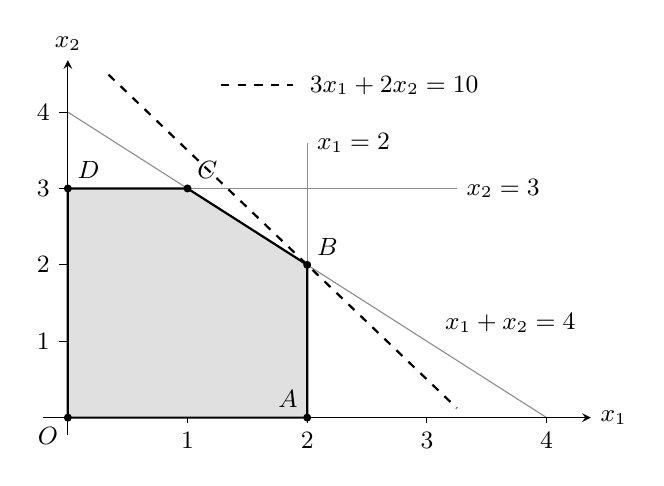
\begin{tikzpicture}[x=1.52cm,y=0.97cm,>=stealth,font=\small]
    \fill[black!12] (0,0)--(2,0)--(2,2)--(1,3)--(0,3)--cycle;
    \draw[black!45] (2,0)--(2,3.6) node[right,text=black] {$x_1=2$};
    \draw[black!45] (0,3)--(3.25,3) node[right,text=black] {$x_2=3$};
    \draw[black!45] (0,4)--(4,0);
    \node[anchor=west] at (3.07,1.24) {$x_1+x_2=4$};
    \draw[thick] (0,0)--(2,0)--(2,2)--(1,3)--(0,3)--cycle;
    \draw[thick,dashed] (0.34,4.49)--(3.25,0.125);
    \draw[thick,dashed] (1.28,4.35)--(1.88,4.35);
    \node[anchor=west] at (1.94,4.35) {$3x_1+2x_2=10$};
    \draw[->] (-0.21,0)--(4.37,0) node[right] {$x_1$};
    \draw[->] (0,-0.23)--(0,4.68) node[above] {$x_2$};
    \foreach \tick in {1,2,3,4}{
      \draw (\tick,0)--(\tick,-0.07) node[below] {$\tick$};
      \draw (0,\tick)--(-0.07,\tick) node[left] {$\tick$};
    }
    \foreach \vertex in {(0,0),(2,0),(2,2),(1,3),(0,3)}
      \fill \vertex circle[radius=1.45pt];
    \node[below left] at (0,0) {$O$};
    \node[above left] at (2,0) {$A$};
    \node[above right] at (2,2) {$B$};
    \node[above right] at (1,3) {$C$};
    \node[above right] at (0,3) {$D$};
  \end{tikzpicture}
  \caption{Допустимая область и оптимальная линия уровня}
  \label{fig:feasible-region}
\end{figure}

Вершины получают пересечением активных граничных прямых.
Для $B$ выполняются $x_1=2$ и $x_1+x_2=4$, откуда $x_2=2$.
Для $C$ выполняются $x_2=3$ и $x_1+x_2=4$, откуда $x_1=1$.
При этом точка $(2,3)$, в которой одновременно достигаются два
индивидуальных предела выпуска, исключается общим ограничением.
В таблице~\ref{tab:worked-example-vertices} приведены значения
целевой функции во всех допустимых вершинах. Наибольшее из них
достигается в вершине $B=(2,2)$.

\begin{table}[htbp]
  \caption{Значения целевой функции в вершинах}
  \label{tab:worked-example-vertices}
  \centering
  \begin{tabular}{lrrrrr}
    \toprule
    Величина & $O$ & $A$ & $B$ & $C$ & $D$ \\
    \midrule
    $x_1$, усл. ед. & 0 & 2 & 2 & 1 & 0 \\
    $x_2$, усл. ед. & 0 & 0 & 2 & 3 & 3 \\
    $f$, ден. ед.   & 0 & 6 & 10 & 9 & 6 \\
    \bottomrule
  \end{tabular}
\end{table}

Результат можно независимо проверить оценкой
\begin{equation}
  f(x_1,x_2)=2(x_1+x_2)+x_1 \le 2\cdot 4+2=10.
  \label{eq:worked-example-bound}
\end{equation}
Равенство в~\eqref{eq:worked-example-bound} возможно только при
$x_1+x_2=4$ и $x_1=2$. Точка $(2,2)$ удовлетворяет
условиям~\eqref{eq:worked-example}, поэтому это единственный
оптимальный план. Максимальная прибыль составляет 10~денежных единиц.

В оптимальном плане общий предел и предел выпуска первого продукта
достигнуты. По второму продукту остаётся запас $3-2=1$~условная единица.
Именно первые две границы использованы в верхней
оценке~\eqref{eq:worked-example-bound}. Коэффициенты $2$ и $1$ в ней
превращают две оценки объёма в оценку общей прибыли.

Ограничения модели могут сохраняться при изменении цели. Если оба
продукта приносят одинаковую положительную прибыль за единицу,
максимизация прибыли сводится к максимизации $x_1+x_2$. Тогда
оптимальна каждая точка отрезка $BC$, то есть $x_1+x_2=4$ при
$1\le x_1\le 2$. Этот случай показывает, как изменение коэффициентов
цели превращает единственный оптимальный план в множество планов.

\subsection{Предварительный выбор метода}

Для дальнейшего решения выбран симплекс-метод. Он переносит идею
сравнения вершин на задачу с произвольным числом переменных и позволяет
проследить, какие ограничения определяют текущий план. Это особенно
важно для учебного примера~\eqref{eq:worked-example}, где выбор вершины
можно сверить графически, перебором и аналитической оценкой.

В симплекс-постановке неравенства $Ax\le b$ записываются как равенства
$Ax+s=b$ с неотрицательными переменными запаса $s$. Если $b\ge 0$,
план $x=0$, $s=b$ даёт начальное допустимое базисное решение,
поскольку столбцы переменных запаса образуют единичную матрицу.
При наличии отрицательной правой части такой старт недопустим.
В двухфазной схеме начальный базис ищут с помощью вспомогательной задачи
первой фазы~\cite{vanderbei2020}. Выбор базиса и правила его смены
относятся к дальнейшему этапу разработки алгоритма.
